\documentclass{beamer}
\usetheme{me} % aalto theme


% Packages for math, language, encoding etc.
\usepackage{tikz, ctable}
\usepackage{bm}
\usepackage[finnish]{babel}
\usepackage[utf8]{inputenc}
\usepackage{graphicx}
\usepackage{xcolor}
\usepackage[absolute,overlay]{textpos}	
\usepackage{amsfonts,amssymb,amsbsy,amsthm,amsmath,mathtools,enumerate,verbatim}
\usepackage{stmaryrd} % double square brackets
\usepackage{color, colortbl}
\usepackage[font=scriptsize]{caption}
\usepackage{csquotes}
\usepackage{tabularray}
\usepackage{hyperref}
\usepackage{datetime}

% Theorem defs
\newtheorem{teoreema}{Lause}
\newtheorem{epateoreema}{Epämuodollinen lause}
\newtheorem{määritelmä}{Määritelmä}

% Notation
\DeclareMathOperator{\var}{Var}
\DeclareMathOperator{\n}{\mathrm N}

% Bibliography and style.
%\usepackage[style=authoryear]{biblatex}
%\addbibresource{sources.bib}
%\setbeamertemplate{bibliography item}{}

%\usepackage[
%  backend=biber,
%  style=authoryear,
%]{biblatex}
%\addbibresource{sources.bib}

% Show greyed table of contents before section.
\AtBeginSection[]
{
    \begin{frame}
        \frametitle{Table of Contents}
        \tableofcontents[currentsection]
    \end{frame}
}
\setcounter{tocdepth}{1}


\AtBeginSubsection[]{
  \begin{frame}
  \vfill
  \centering
  \begin{beamercolorbox}[sep=8pt,center,shadow=true,rounded=true]{subtitle}
    \usebeamerfont{subtitle}\insertsubsectionhead\par%
  \end{beamercolorbox}
  \vfill
  \end{frame}
}

% Info about presentation
\title{Keskeinen raja-arvolause ja sen sovellukset liiketoiminnassa}
\subtitle{\url{https://github.com/perej1/clt-teaching}}
\author{Jaakko Pere}

\newdate{date}{25}{3}{2025}
\date{\displaydate{date}}


% Page number
% \setbeamertemplate{footline}[frame number]

%%%%%%%%%%%%%%%%%%%%%%%%%%%%%%%%%%%%%%%%%%%%%%%%%%%%%%%%%%%%%%%%%%%%%%%%%%%%%%%
%%%%%%%%%%%%%%%%%%%%%%%%%%%%%%% DOCUMENT BEGINS %%%%%%%%%%%%%%%%%%%%%%%%%%%%%%%
%%%%%%%%%%%%%%%%%%%%%%%%%%%%%%%%%%%%%%%%%%%%%%%%%%%%%%%%%%%%%%%%%%%%%%%%%%%%%%%
\begin{document}

\frame{\titlepage}

%%%%%%%%%%%%%%%%%%%%%%%%%%%%%%%%%%%

\begin{frame}{Kohdeyleisö}
  \begin{itemize}
    \item Ensimmäisen ja toisen vuoden kandiopiskelijat (lukion matematiikka).
    \pause
    \item Kurssilla on jo käsitelty seuraavat käsitteet:
    \begin{itemize}
      \item Satunnaismuuttuja
      \item Odotusarvo
      \item Varianssi
      \item Estimaattori
      \item Suurten lukujen laki
    \end{itemize}
  \end{itemize}
\end{frame}

%%%%%%%%%%%%%%%%%%%%%%%%%%%%%%%%%%%

\begin{frame}{Luennon sisältö}
  \tableofcontents
\end{frame}

%%%%%%%%%%%%%%%%%%%%%%%%%%%%%%%%%%%

\section{Moraali}

%%%%%%%%%%%%%%%%%%%%%%%%%%%%%%%%%%%

\begin{frame}{Suurten lukujen laki}
  Olkoon $X_1, \ldots, X_n$ riippumattomia ja samoin jakautuneita
  satunnaismuuttujia niin, että $\mu = \mathbb{E}\left(X_1\right)\in (-\infty,
  \infty)$.
  \pause
  Tällöin suurten lukujen laki kertoo, että suurilla $n$
  \begin{equation*}
    \bar X = \frac{1}{n}\sum_{i=1}^{n} X_i \approx \mathbb{E}\left(X_1\right).
  \end{equation*}
  \pause
  Toisin sanoen keskiarvo estimoi odotusarvoa.
  \begin{itemize}
    \item[]
  \end{itemize}
  \pause
  \textcolor{red}{Tarkemmin ilmaistuna
  $\lim_{n\to\infty}\mathbb{P}\left(\left|\bar X - \mu\right| >
  \varepsilon\right) = 0$ kaikilla $\varepsilon > 0$.}
\end{frame}

%%%%%%%%%%%%%%%%%%%%%%%%%%%%%%%%%%%

\begin{frame}{Ongelma}
  \begin{itemize}
    \item Suurten lukujen laki ei kerro mitään siitä kuinka hyvin keskiarvo
    estimoi odotusarvoa.
    \pause
    \item Voidaanko keskiarvon jakaumasta sanoa jotain edes suurilla
    otosko'oilla $n$?
  \end{itemize} 
\end{frame}

%%%%%%%%%%%%%%%%%%%%%%%%%%%%%%%%%%%

\begin{frame}{Esimerkki: luottokorttipetokset}
  \begin{itemize}
    \item Otos sisältää luottokorttitapahtumia Euroopasta syyskuulta 2013.
    Tapahtumia kirjattiin kahdelta päivältä (Lähde:
    \href{https://www.kaggle.com/datasets/mlg-ulb/creditcardfraud?resource=download}{\textcolor{red}{Kaggle}}).
    \pause
    \item Luottokorttitapahtumia on yhteensä 284 807, joista 492 luokiteltiin
    petoksiksi.
    \pause
    \item Estimaatti luottokorttipetoksen todennäköisyydelle on $492 / 284
    807\approx 0.0017$.
    \pause
    \item Kuinka varma voin olla siitä, että saatu piste-estimaatti on lähellä
    populaatisuuretta?
  \end{itemize}
\end{frame}

%%%%%%%%%%%%%%%%%%%%%%%%%%%%%%%%%%%

\begin{frame}{Simulaatio}
  \begin{enumerate}
    \item Simuloi otos riippumattomia ja samoin jakauneita havaintoja $x_1,
    \ldots, x_n$ (otoskoko on $n$). Laske keskiarvo
    \begin{equation*}
      \bar x = \frac{1}{n}\sum_{i=1}^n x_i.
    \end{equation*}
    \pause
    \item Toista yllä oleva toimenpide $m = 1000$ kertaa. Näin meillä on $m$
    keskiarvoa.
    \pause
    \item Piirrä histogrammi keskiarvoista.
  \end{enumerate}
\end{frame}

%%%%%%%%%%%%%%%%%%%%%%%%%%%%%%%%%%%

\begin{frame}
  \begin{itemize}
    \item Ensin simuloimme otoksia tasajakaumasta $U[0,1]$ välillä 0-1 (jakauman
    odotusarvo on $0.5$). Kyseisen tasajakauman tiheysfunktio on
    \begin{equation*}
      f(x) =
      \begin{cases}
        1, &\textnormal{kun}\quad x\in[a,b], \\
        0, &\textnormal{muulloin}. 
      \end{cases}
    \end{equation*}
  \end{itemize}
\end{frame}

%%%%%%%%%%%%%%%%%%%%%%%%%%%%%%%%%%%

\begin{frame}
  \begin{center}
    \begin{figure}
      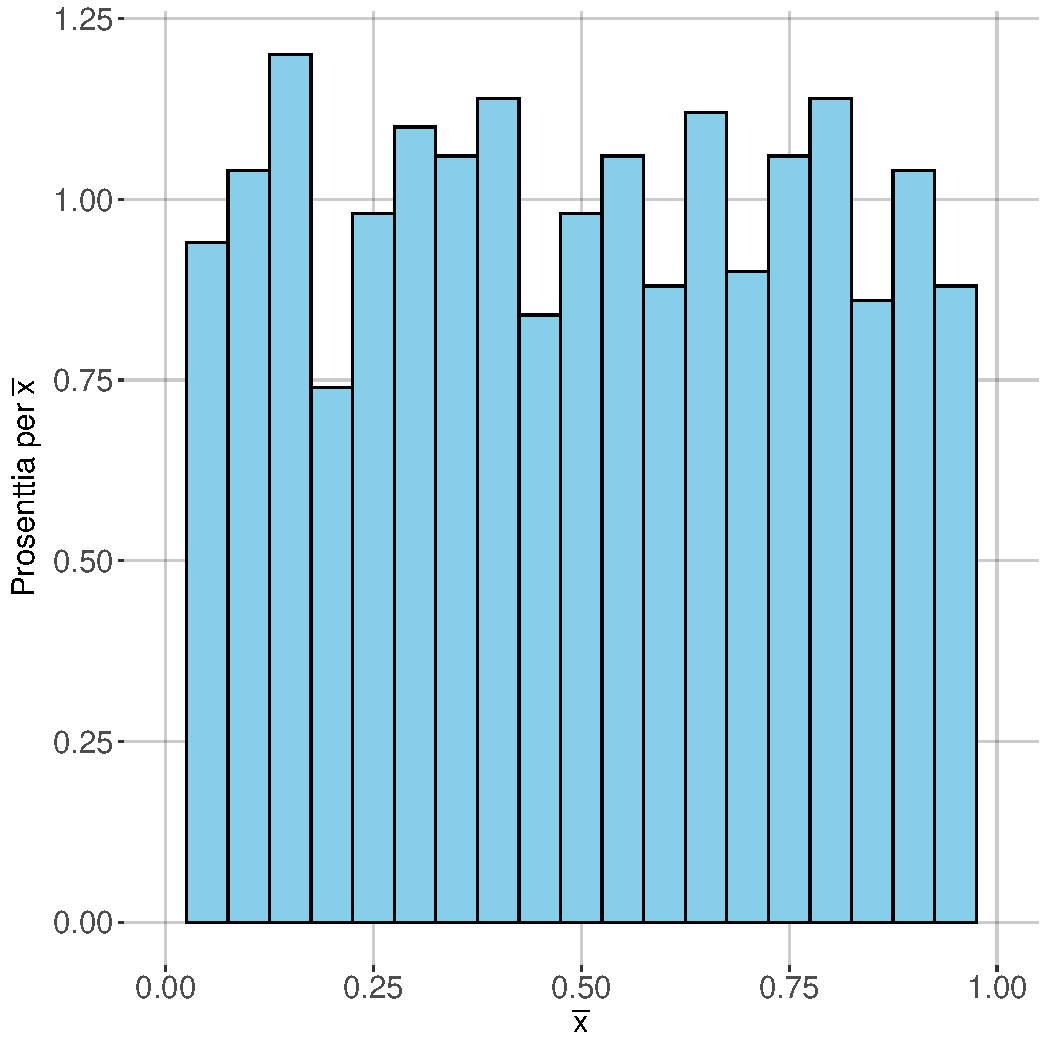
\includegraphics[width=0.7\textwidth, height=0.7\textwidth]{unif-n-1.pdf}
      \caption{Tasajakauma $U[0,1]$, $n = 1$ ja $m = 1000$.}
    \end{figure}
  \end{center}
\end{frame}

%%%%%%%%%%%%%%%%%%%%%%%%%%%%%%%%%%%

\begin{frame}
  \begin{center}
    \begin{figure}
      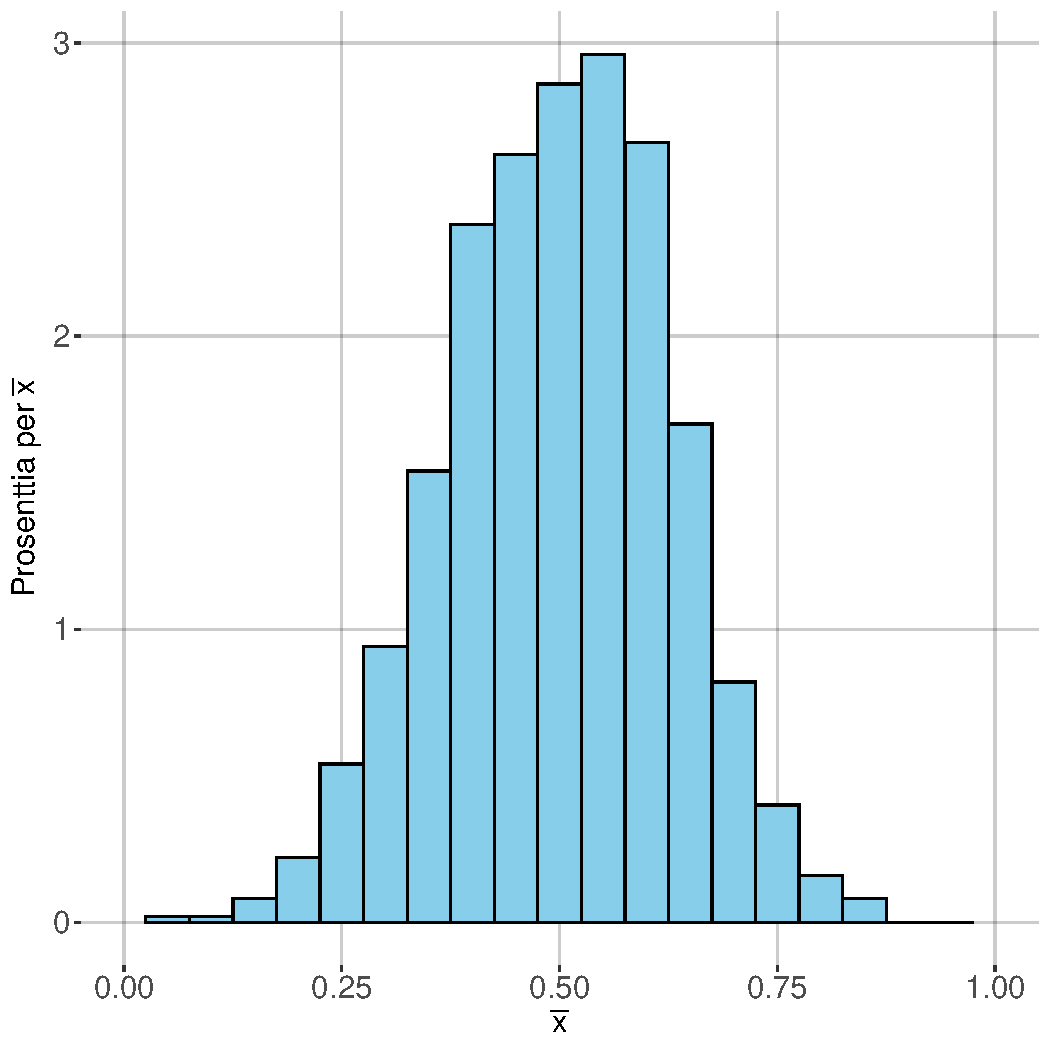
\includegraphics[width=0.7\textwidth, height=0.7\textwidth]{unif-n-5.pdf}
      \caption{Tasajakauma $U[0,1]$, $n = 5$ ja $m = 1000$.}
    \end{figure}
  \end{center}
\end{frame}

%%%%%%%%%%%%%%%%%%%%%%%%%%%%%%%%%%%

\begin{frame}
  \begin{center}
    \begin{figure}
      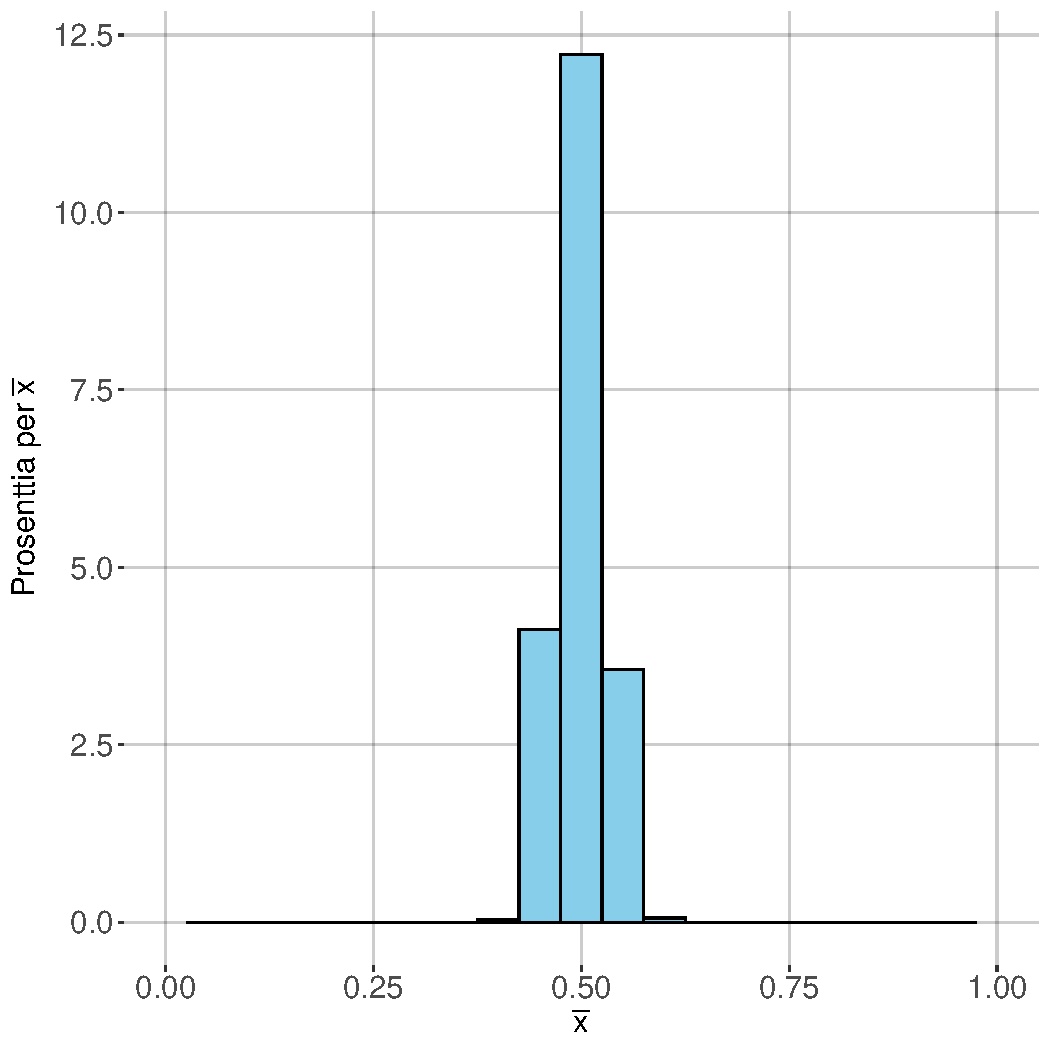
\includegraphics[width=0.7\textwidth, height=0.7\textwidth]{unif-n-100.pdf}
      \caption{Tasajakauma $U[0,1]$, $n = 100$ ja $m = 1000$.}
    \end{figure}
  \end{center}
\end{frame}

%%%%%%%%%%%%%%%%%%%%%%%%%%%%%%%%%%%

\begin{frame}
  \begin{itemize}
    \item Seuraavaksi simuloimme otoksia eksponenttijakaumasta $\mathrm{Exp}(1)$
    skaalaparametrilla $\lambda = 1$ (jakauman odotusarvo on $1$). Kyseisen
    eksponentijakauman tiheysfunktio on
    \begin{equation*}
      f(x) =
      \begin{cases}
        e^{-x}, &\textnormal{kun}\quad x\in[0,\infty), \\
        0, &\textnormal{muulloin}. 
      \end{cases}
    \end{equation*}
  \end{itemize}
\end{frame}

%%%%%%%%%%%%%%%%%%%%%%%%%%%%%%%%%%%

\begin{frame}
  \begin{center}
    \begin{figure}
      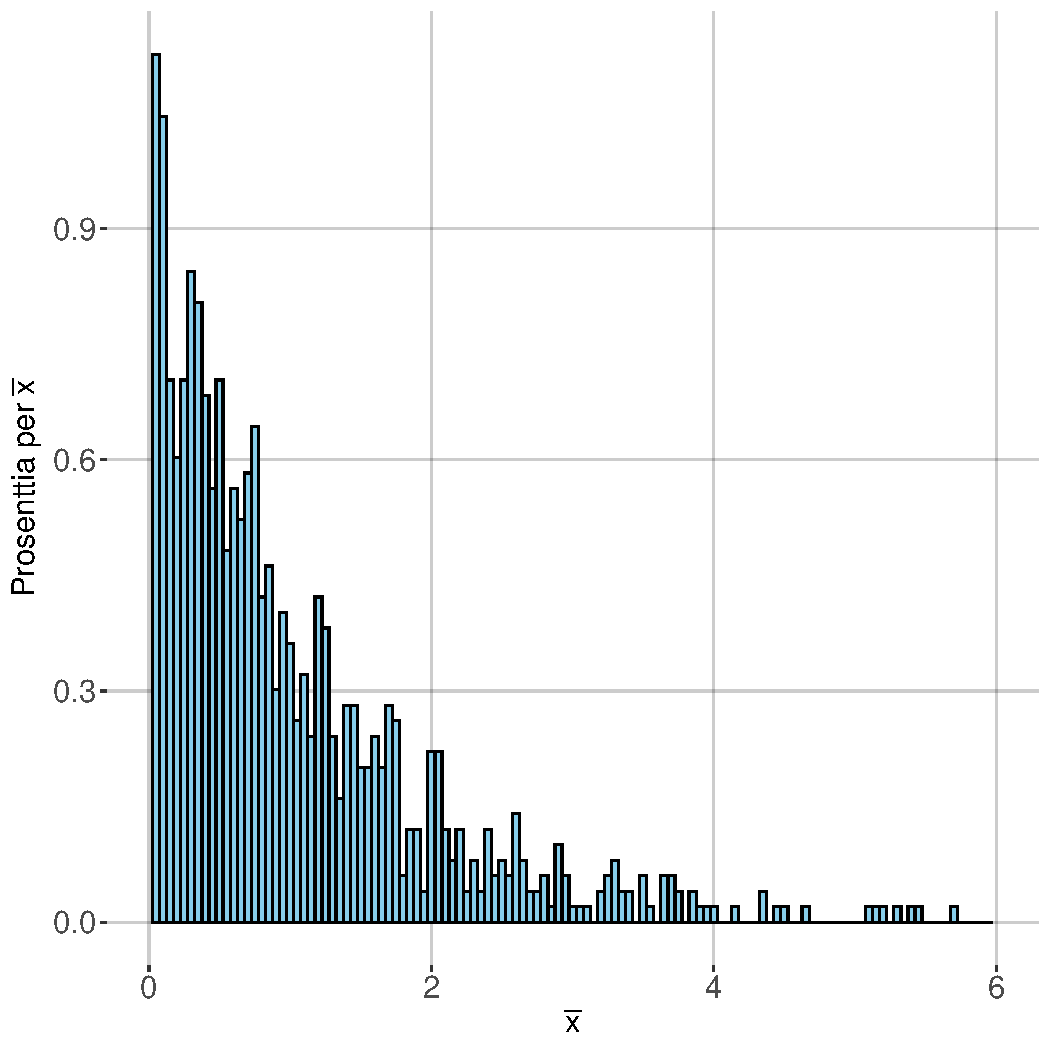
\includegraphics[width=0.7\textwidth, height=0.7\textwidth]{exp-n-1.pdf}
      \caption{Eksponenttijakauma $\mathrm{Exp}\left(1\right)$, $n = 1$ ja $m = 1000$.}
  \end{figure}
\end{center}
\end{frame}

%%%%%%%%%%%%%%%%%%%%%%%%%%%%%%%%%%%

\begin{frame}
  \begin{center}
    \begin{figure}
      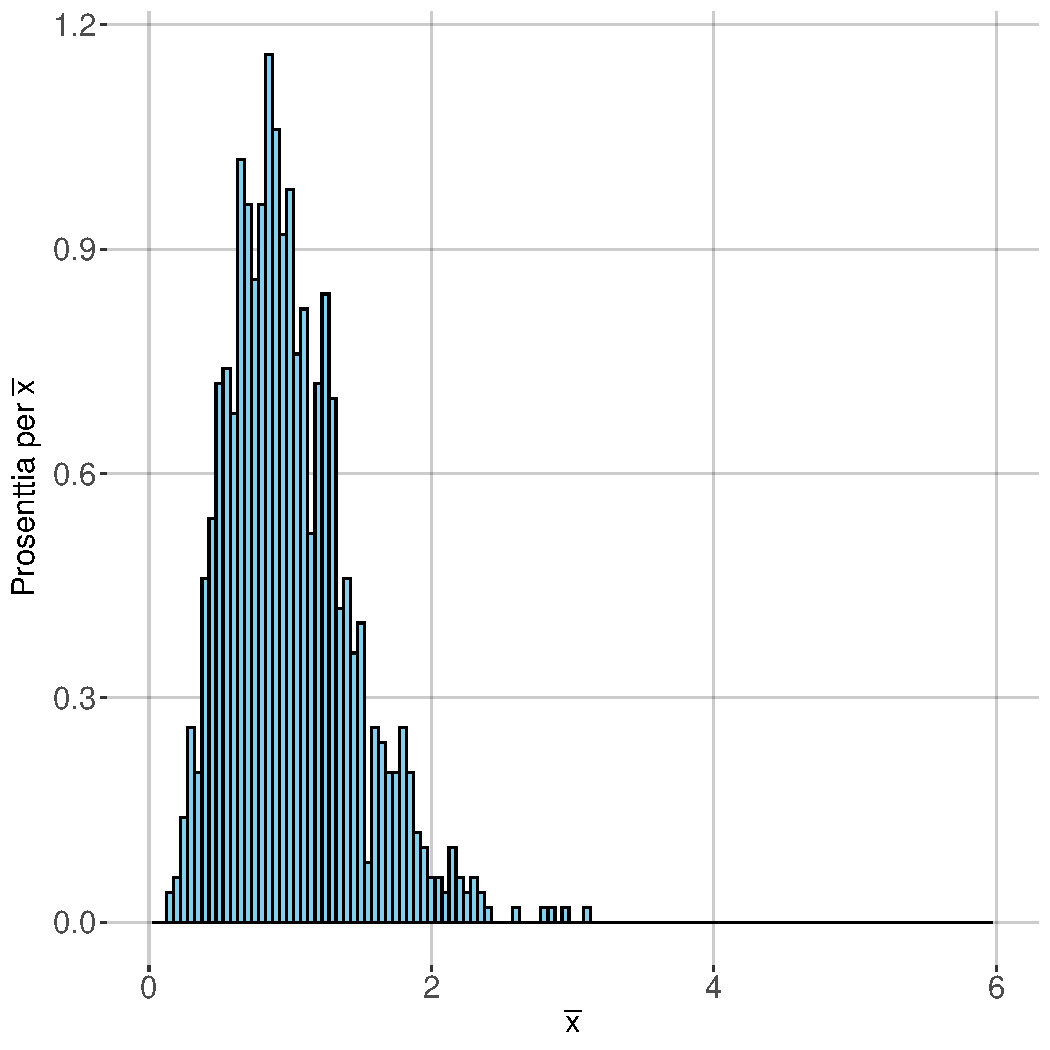
\includegraphics[width=0.7\textwidth, height=0.7\textwidth]{exp-n-5.pdf}
      \caption{Eksponenttijakauma $\mathrm{Exp}\left(1\right)$, $n = 5$ ja $m = 1000$.}
  \end{figure}
\end{center}
\end{frame}

%%%%%%%%%%%%%%%%%%%%%%%%%%%%%%%%%%%

\begin{frame}
  \begin{center}
    \begin{figure}
      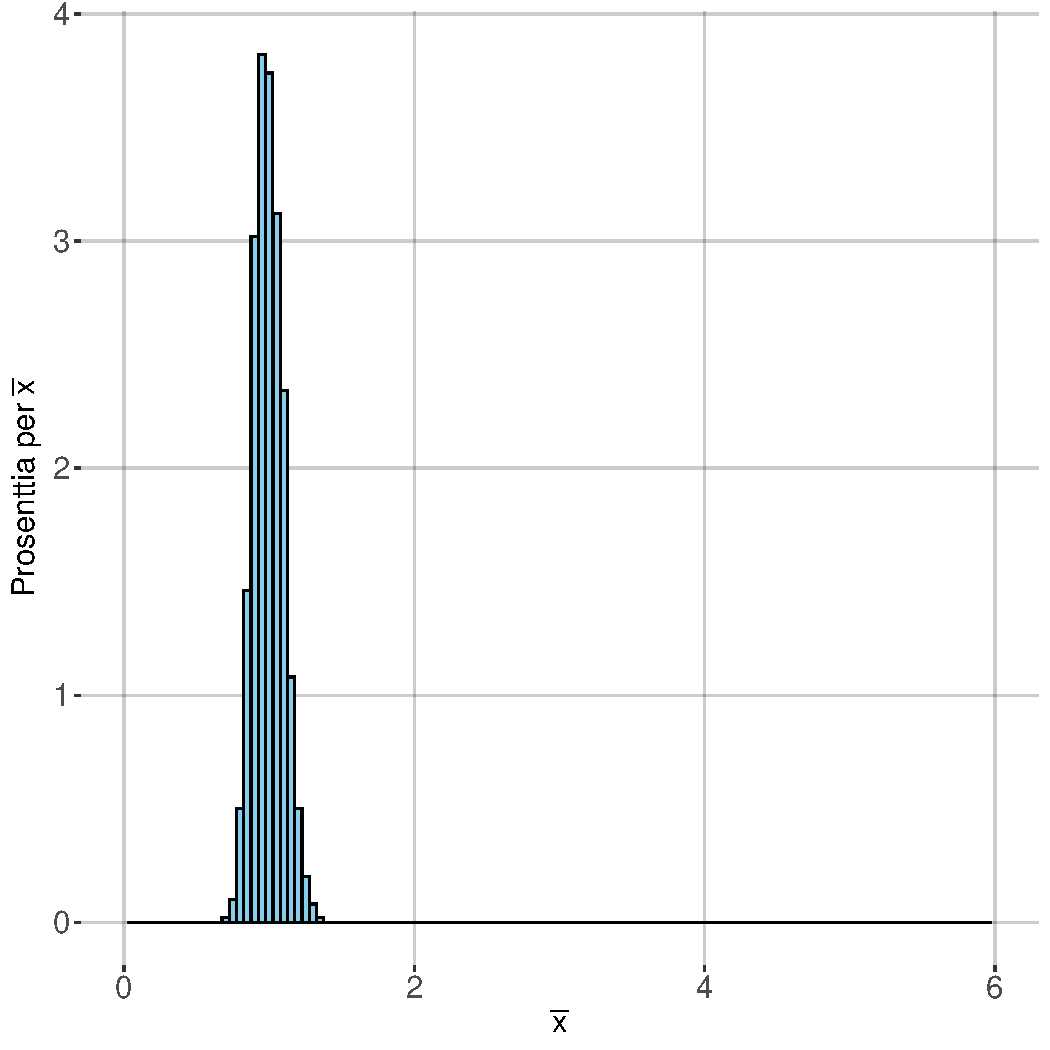
\includegraphics[width=0.7\textwidth, height=0.7\textwidth]{exp-n-100.pdf}
      \caption{Eksponenttijakauma $\mathrm{Exp}\left(1\right)$, $n = 100$ ja $m = 1000$.}
  \end{figure}
\end{center}
\end{frame}

%%%%%%%%%%%%%%%%%%%%%%%%%%%%%%%%%%%

\begin{frame}{Opetustavoitteet}
  Luennon jälkeen osaamme
  \begin{enumerate}
    \item approksimoida todennäköisyyksiä klassisen keskeisen raja-arvolauseen
    avulla ja
    \pause
    \item muodostaa likiarvoisen luottamusvälin odotusarvolle perustuen
    keskeiseen raja-arvolauseeseen.
  \end{enumerate}
\end{frame}

%%%%%%%%%%%%%%%%%%%%%%%%%%%%%%%%%%%

\section{Normaalijakauma}

\begin{frame}
  Normaalijakauma on absoluuttisesti jatkuva jakauma. Merkitsemme
  normaalijakaumaa parametrein $\mu\in(-\infty, \infty)$ ja
  $\sigma^2\in(0,\infty)$ notaatiolla $\n\left(\mu, \sigma^2\right)$. Jakauman
  $\n\left(\mu, \sigma^2\right)$ tiheysfunktio on
  \begin{equation*}
    f(x) = \frac{1}{\sqrt{2\pi\sigma^2}} e^{-\frac{\left(x-\mu\right)^2}
    {2\sigma^2}}.
  \end{equation*}
  \pause
  \begin{itemize}
    \item[]
  \end{itemize}
  Tällöin normaalijakauman kertymäfunktio voidaan esittää tiheysfunktion avulla
  \begin{equation*}
    F\left(x\right) = \int_{-\infty}^{x} f(t)\,\mathrm{d}t.
  \end{equation*}
\end{frame}

%%%%%%%%%%%%%%%%%%%%%%%%%%%%%%%%%%%

\begin{frame}
  \begin{center}
    \begin{figure}
      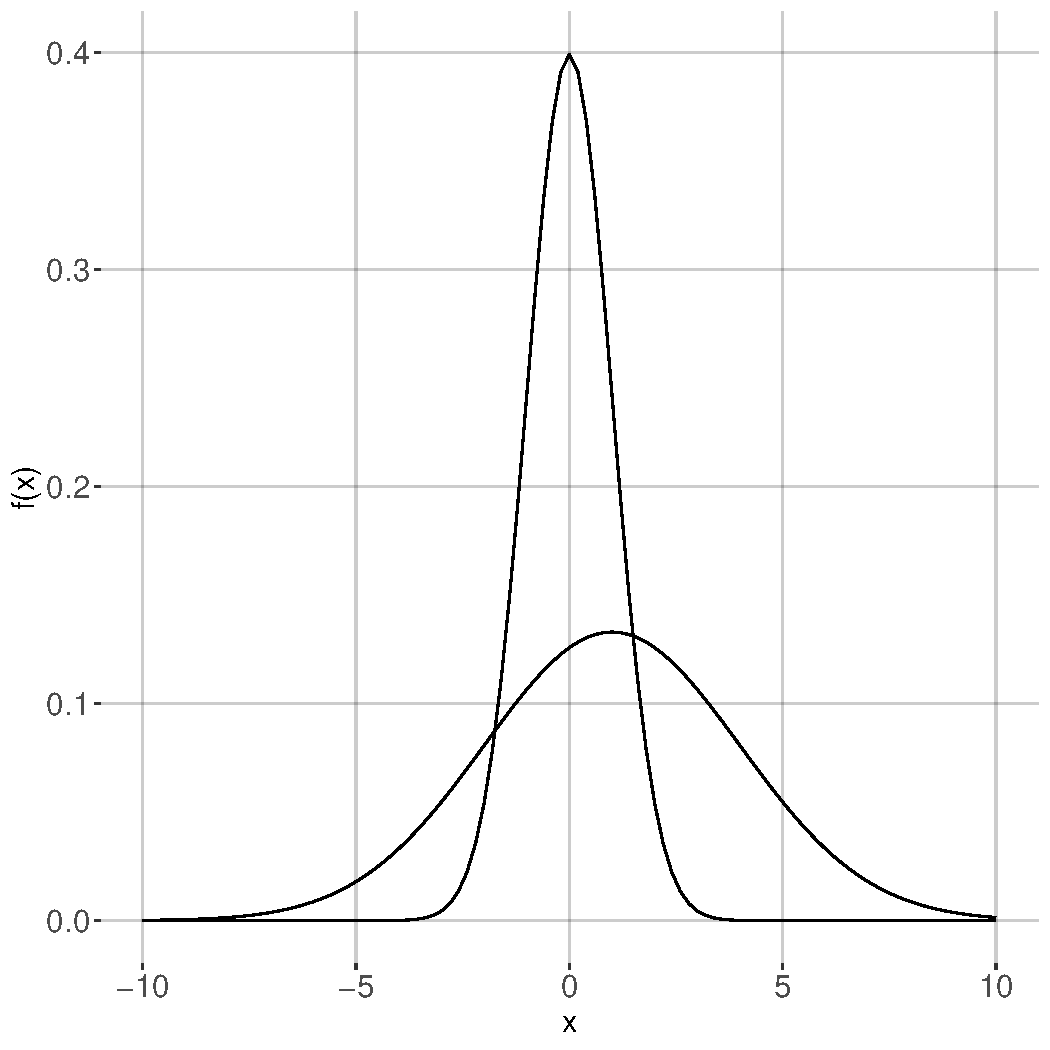
\includegraphics[width=0.7\textwidth, height=0.7\textwidth]{normal}
      \caption{Normaalijakaumat $\n\left(0,1\right)$ (katkoviiva) ja $\n\left(1, 9\right)$ (jatkuva viiva).}
    \end{figure}
  \end{center}
\end{frame}

%%%%%%%%%%%%%%%%%%%%%%%%%%%%%%%%%%%

\section{Keskeinen raja-arvolause}

%%%%%%%%%%%%%%%%%%%%%%%%%%%%%%%%%%%

\begin{frame}
  \begin{teoreema}
    Olkoon $X_1, X_2, \ldots, X_n$ riippumattomia ja samoin jakautuneita
    satunnaismuuttujia niin, että $0 < \var\left(X_1\right) < \infty$.
    Merkitsemme $\bar X = \frac{1}{n}\sum_{i = 1}^n X_i$, $\mu =
    \mathbb{E}\left(X_1\right)$ ja $\sigma = \sqrt{\var\left(X_1\right)}$.
    Tällöin, kun otoskoko $n$ on suuri, niin
    \begin{equation*}
      \tilde X = \sqrt{n}\frac{\bar X - \mu}{\sigma}
    \end{equation*}
    noudattaa likimain standardinormaalijakaumaa $\n\left(0, 1\right)$,
    \pause
    \begin{equation*}
      \mathbb{P}\left(\tilde X \leq x\right) \approx
      \int_{-\infty}^x \frac{1}{\sqrt{2\pi}}e^{-t^2/2}\,\mathrm{d}t =:
      \Phi\left(x\right).
    \end{equation*}
  \end{teoreema}
\end{frame}

%%%%%%%%%%%%%%%%%%%%%%%%%%%%%%%%%%%

\section{Sovellukset}

%%%%%%%%%%%%%%%%%%%%%%%%%%%%%%%%%%%

\subsection{Todennäköisyyksien approksimointi}

%%%%%%%%%%%%%%%%%%%%%%%%%%%%%%%%%%%

\begin{frame}
  Keskeisen raja-arvolauseen oletusten pätiessä $\tilde X$ noudattaa likimain
  normaalijakaumaa, jossa
  \begin{equation*}
    \tilde X = \sqrt{n}\frac{\frac{1}{n}
    \overbrace{\sum_{i=1}^n X_i}^{=S_n} - \mu}{\sigma}
    = \frac{S_n - n\mu}{\sqrt{n}\sigma}.
  \end{equation*}
  \pause
  Tällöin
  \begin{equation*}
    \mathbb{P}\left(S_n\leq x\right) = \mathbb{P}
    \left(\underbrace{\frac{S_n - n\mu}{\sqrt{n}\sigma}}_{= \tilde X}\leq
    \frac{x - n\mu} {\sqrt{n}\sigma}\right)\approx \Phi\left(\frac{x - n\mu}
    {\sqrt{n}\sigma}\right).
  \end{equation*}
\end{frame}

%%%%%%%%%%%%%%%%%%%%%%%%%%%%%%%%%%%

\begin{frame}{Esimerkki}
  \begin{itemize}
    \item $X_1, \ldots, X_n$ ovat riippumattomia satunnaismuuttujia Bernoullin
    jakaumasta, $\mathbb{P}\left(X_1 = 1\right) = p$ ja $\mathbb{P}\left(X_1 =
    0\right) = 1-p$.
    \pause
    \item Voimme laskea, että $\mu = \mathbb{E}\left(X_1\right) = p$ ja
    $\sigma^2 = \var\left(X_1\right) = p(1-p)$.
  \end{itemize}
  \pause
  Saamme approksimaation
  \begin{equation*}
    \mathbb{P}\left(S_n \leq x\right) \approx \Phi\left(\frac{x - np}
    {\sqrt{np(1-p)}}\right).
  \end{equation*}
\end{frame}

%%%%%%%%%%%%%%%%%%%%%%%%%%%%%%%%%%%

\begin{frame}{Esimerkki: luottokorttipetokset}
  \begin{itemize}
    \item Oletetaan, että tiedämme petoksen todennäköisyyden olevan $p =
    0.0016$.
    \item Mikä on todennäköisyys havaita vähintään $x = 492$ petosta, kun
    luottokorttitapahtumia oli kokonaisuudessaan $n = 284807$?
    \item Approksimoimme
    \begin{equation*}
      \mathbb{P}\left(S_n \geq x\right) \approx 1 - \Phi\left(\frac{x - np}
      {\sqrt{np(1-p)}}\right).
    \end{equation*}
  \end{itemize}
  
\end{frame}

%%%%%%%%%%%%%%%%%%%%%%%%%%%%%%%%%%%

\subsection{Likiarvoinen luottamusväli}

%%%%%%%%%%%%%%%%%%%%%%%%%%%%%%%%%%%

\begin{frame}{Luottamusvälin määritelmä odotusarvolle}
  \begin{itemize}
    \item Oletetaan, että $X$ on satunnismuuttuja odotusarvolla $\mu =
    \mathbb{E}\left(X\right)\in(-\infty, \infty)$. Olkoon $\bm X = (X_1, \ldots,
    X_n)$ satunnaismuuttujan $X$ havaintoja.
    \pause
    \item Luottamustason $1-\alpha$ luottamusväli on satunnaisväli
    $\left[\ell\left(\bm X\right), u\left(\bm X\right)\right]$, jolle pätee
    \begin{equation*}
      \mathbb{P}\left(\mu\in\left[\ell\left(\bm X\right), u\left(\bm
      X\right)\right]\right) \geq 1 - \alpha.
    \end{equation*}
  \end{itemize}
\end{frame}

%%%%%%%%%%%%%%%%%%%%%%%%%%%%%%%%%%%

\begin{frame}{Luottamusvälin approksimointi (1)}
  Oletetaan, että satunnaismuuttujan $X$ varianssi $0 < \sigma^2 < \infty$ on
  tiedossa. Tällöin keskeisen raja-arvolauseen mukaan
  \begin{equation*}
    \mathbb{P}\left(z_{\ell} \leq \sqrt{n}\frac{\mu - \bar X}{\sigma}
    \leq z_u\right) \approx 1 - \alpha,
  \end{equation*}
  \pause
  jossa väli $[z_\ell, z_u]$ valitaan niin, että
  \begin{equation*}
    \Phi(z_u) - \Phi(z_\ell) = 1-\alpha.
  \end{equation*}
  Yllä $F$ on jakauman $\n\left(0,1\right)$ kertymäfunktio.
\end{frame}

%%%%%%%%%%%%%%%%%%%%%%%%%%%%%%%%%%%

\begin{frame}{Luottamusvälin approksimointi (2)}
  Valitsemalla esimerkiksi $z_u = z_{1 - \alpha/2}$ ja $z_\ell = -z_u$ päädymme
  seuravaan luottamusväliin
  \begin{equation*}
    \left[\bar X - \frac{\sigma z_{1 - \alpha/2}}{\sqrt{n}},
    \bar X + \frac{\sigma z_{1 - \alpha/2}}{\sqrt{n}}\right].
  \end{equation*}
  \pause
  Käytännössä yleensä (tuntematon) keskihajonta korvataan vielä
  otoskeskihajonnalla $\hat\sigma$, sillä suurten lukujen lain perusteella
  $\hat\sigma\approx\sigma$. Päädymme luottamusväliin
  \begin{equation*}
    \left[\bar X - \frac{\hat\sigma z_{1 - \alpha/2}}{\sqrt{n}},
    \bar X + \frac{\hat\sigma z_{1 - \alpha/2}}{\sqrt{n}}\right].
  \end{equation*}
\end{frame}

%%%%%%%%%%%%%%%%%%%%%%%%%%%%%%%%%%%

\begin{frame}{Esimerkki: luottokorttipetokset}
  \begin{itemize}
    \item Otos sisältää luottokorttitapahtumia syyskuulta 2013. Tapahtumia
    kirjattiin kahdelta päivältä
    (Lähde: \href{https://www.kaggle.com/datasets/mlg-ulb/creditcardfraud?resource=download}{\textcolor{red}{Kaggle}}).
    \pause
    \item Luottokorttitapahtumia on yhteensä 284 807, joista 492 luokiteltiin
    petoksiksi.
    \pause
    \item Tavoite: Estimoidaan 95\% luottamusväli petoksien osuudelle
    luottokorttitapahtumista.
  \end{itemize}
\end{frame}

%%%%%%%%%%%%%%%%%%%%%%%%%%%%%%%%%%%

\begin{frame}{Malli}
  \begin{itemize}
    \item Satunnaismuuttuja $X$ noudattaa Bernoullijakaumaa tuntemattomalla
    parametrilla $p$, jossa $p$ on petoksen todennäköisyys.
    \item $\mathbb{P}\left(X = 1\right) = p$ ja $\mathbb{P}\left(X = 0\right) =
    1 - p$, jossa tapahtuma $\{X = 1\}$ indikoi petosta ja $\{X = 0\}$ vastaa
    normaalia luottokorttitapahtumaa.
    \item Havainnot $x_1, \ldots x_{284807}$ ovat binäärisiä (0 tai 1).
    Oletamme, että havainnot ovat riippumattomia ja samoin jakautuneita.
  \end{itemize}
\end{frame}

%%%%%%%%%%%%%%%%%%%%%%%%%%%%%%%%%%%

\begin{frame}{Ratkaisu}
  \begin{itemize}
    \item Voimme laskea $\mathbb{E}\left(X\right) = p$ ja $\var\left(X\right) =
    p(1-p)$.
    \item Suurten lukujen lain mukaan $p \approx \hat p =
    \frac{1}{n}\sum_{i=1}^{284807} x_i$.
    \item Joten voimme approksimoida $95\%$ luottamusvälin seuraavasti
    \begin{equation*}
      \left[\hat p - z_{1 - \alpha/2}\sqrt{\frac{\hat p(1-\hat p)}{n}},
      \hat p + z_{1 - \alpha/2}\sqrt{\frac{\hat p(1-\hat p)}{n}}\right].
    \end{equation*}
  \end{itemize}
\end{frame}

%%%%%%%%%%%%%%%%%%%%%%%%%%%%%%%%%%%

\begin{frame}{Ratkaisu (2)}
  Sijoittamalla lukuarvot
  \begin{itemize}
    \item $\hat p\approx 0.0017$, (\textsf{R} komento \texttt{mean(data)}) ja
    \item $z_{1 - \alpha / 2} \approx 1.96$ (\textsf{R} komento \texttt{qnorm(1
    - 0.05 / 2)})
  \end{itemize}
  saamme luottamusväliksi
  \begin{equation*}
    \approx \left[0.0016, 0.0019\right].
  \end{equation*}
  \pause
  \begin{itemize}
    \item[]
  \end{itemize}
  Luottamusvälin laskemiseen liittyvät yksityiskohdat löytyvät skriptistä
  \texttt{credit.R}. 
\end{frame}

\begin{frame}{Tiivistelmä}
  Sovelsimme keskeistä raja-arvolausetta luottokorttipetoksiin
  \begin{enumerate}
    \item approksimoimalla petoksien määrän todennäköisyyttä ja
    \item laskemalla likiarvoistettuja luottamusvälejä petoksen
    todennäköisyydelle.
  \end{enumerate}
\end{frame}
\end{document}
